\section{User Datagram Protocol}

\subsection{Protocolos de Transporte}

\begin{definicion}{Protocolos de Transporte} 
    Proveen \textbf{comunicación lógica entre procesos de aplicación} ejecutándose en distintos hosts. Se implementan sólo en los \textbf{extremos}, no en los dispositivos intermedios. 

    Reciben los datos de la capa de aplicación, los divide en pedazos y les agrega una nueva cabecera. Proveen multiplexación y demultiplexación de aplicaciones.
    
    Actúan como una interface entre la \textbf{aplicación} y el \textbf{sistema operativo}.
\end{definicion} 

\subsubsection{Puertos}

Los puertos son una abstracción identificada con un número, cuya implementación depende de cada sistema operativo. 

Identifican unívocamente la \textbf{aplicación} transmisora y receptora. 

Hay tres tipos de puertos:

\begin{itemize}[label=\textcolor{acento}{$\bullet$}]
    \item \textbf{Well-known:} \texttt{0 ... 1023}.
    \item \textbf{Registered:} \texttt{1024 ... 49151}.
    \item \textbf{Ephimeral:} \texttt{49152 ... 65535}.
\end{itemize}

\subsection{Sockets}

\begin{definicion}{Definición}
    Los sockets son la interface entre la capa de aplicación y la capa de transporte, mediante la cual los procesos se comunican escribiendo y leyendo.
\end{definicion}

La \textbf{dirección de un socket} está compuesta por: 

\begin{itemize}[label=\textcolor{acento}{$\bullet$}]
    \item Protocolo
    \item Proceso local
    \item Dirección local
\end{itemize}

Y la \textbf{sesión} es: \texttt{[protocolo, proceso local, dirección local, proceso remoto, dirección remota]}

\begin{nota}{\emph{Recordar}}
    En resumen, la capa de transporte aporta comunicación lógica entre procesos mediante puertos y sockets.
\end{nota}

\subsection{Características de UDP}

\begin{definicion}{UDP}
    UDP es un protocolo de transporte \textbf{Best-Effort}, sin conexión: no hay ni handshake y los datagramas son independientes. No provee mecanismos de control de errores, flujo o congestión.
\end{definicion}

La estructura del datagrama es la siguiente.

\begin{figure}[htbp]
    \centering
    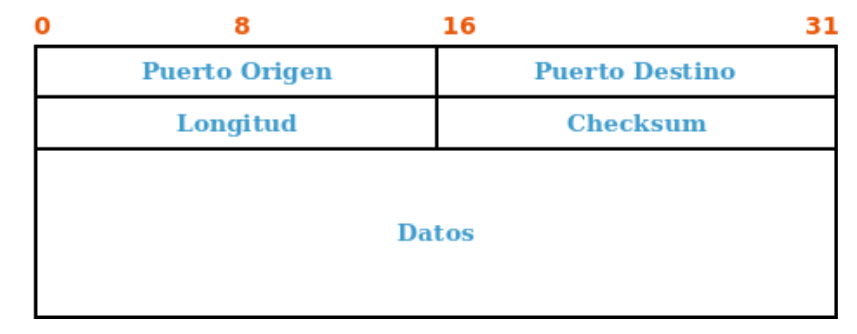
\includegraphics[width=0.7\textwidth]{capitulos/udp/imagenes/datagrama-udp.png}
    \caption{Datagrama de UDP}
    \label{fig:datagrama-udp}
\end{figure}

El tamaño de la \textbf{cabecera} siempre es de \texttt{8 Bytes}, y el checksum es opcional. 

UDP también tiene una \textbf{pseudocabecera} que se añade al principio del datagrama para el cálculo del checksum, pero \textbf{no se envía}. Sirve para comprobar que IP no se haya equivocado en la entrega del datagrama. 

El datagrama de UDP se \textbf{encapsula} en un paquete IP. 

